\documentclass[tikz]{standalone}
\usetikzlibrary{arrows.meta}
\usetikzlibrary{decorations.pathmorphing}
\begin{document}

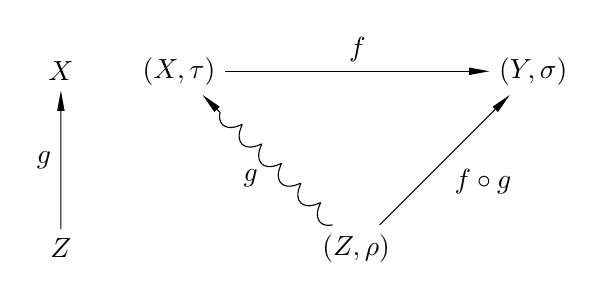
\begin{tikzpicture}[-latex, arrows={-Triangle[angle=20:5pt,scale=1.5]}, scale=1.5]
	\node (X) at (0,0) {\((X, \tau)\)};
	\node (Y) at (3,0) {\((Y, \sigma)\)};
	\node (Z) at (1.5,-1.5) {\((Z, \rho)\)};

	\draw (X) to node [above] {\(f\)} (Y);
	\draw [decorate, decoration={coil}] (Z) to node [below left] {\(g\)} (X);
	\draw (Z) to node [below right] {\(f \circ g\)} (Y);

	\node (A) at (-1,-1.5) {\(Z\)};
	\node (B) at (-1,0) {\(X\)};
	\draw (A) -- node [left] {\(g\)} (B);
\end{tikzpicture}

\begin{tikzpicture}[-latex, arrows={-Triangle[angle=20:5pt,scale=1.5]}, scale=1.5]
	\node (X) at (0,0) {\((X, \tau)\)};
	\node (Y) at (3,0) {\((Y, \sigma)\)};
	\node (Z) at (1.5,-1.5) {\((Z, \rho)\)};

	\draw (X) to node [above] {\(f\)} (Y);
	\draw  (Z) to node [below left] {\(g\)} (X);
	\draw (Z) to node [below right] {\(f \circ g\)} (Y);
\end{tikzpicture}

\end{document}
